%!  pour pdfLatex
\documentclass{beamer}

%\usepackage[pdftex]{graphicx,color}
%\usepackage[pdftex,colorlinks={true},urlcolor={blue},pdfauthor={remy Nicolai}]{hyperref}

\usepackage[utf8]{inputenc}
\usepackage[T1]{fontenc}
\usepackage{lmodern}
\usepackage[frenchb]{babel}

\usetheme{Warsaw}

%\usepackage{fancyhdr}
%\pagestyle{fancy}

%\usepackage{floatflt}
\usepackage{maths}

\usepackage{parcolumns}
\setlength{\parindent}{0pt}

%\usepackage{caption}
%\usepackage{subcaption}

\usepackage[french,ruled,vlined]{algorithm2e}
\SetKwComment{Comment}{\#}{}
\SetKwFor{Tq}{tant que}{}{}
\SetKwFor{Pour}{pour}{}{}
\DontPrintSemicolon
\SetAlgoLined

\usepackage{listings}
\lstset{language=Python,frame=single}

%pr{\'e}sentation des compteurs de section, ...
\makeatletter
\renewcommand{\thesection}{\Roman{section}.}
\renewcommand{\thesubsection}{\arabic{subsection}.}
\renewcommand{\thesubsubsection}{\arabic{subsubsection}.}
%\renewcommand{\labelenumii}{\theenumii.}
\makeatother


\newtheorem*{thm}{Théorème}
\newtheorem{thmn}{Théorème}
\newtheorem*{prop}{Proposition}
\newtheorem{propn}{Proposition}
\newtheorem*{pa}{Présentation axiomatique}
\newtheorem*{propdef}{Proposition - Définition}
\newtheorem*{lem}{Lemme}
\newtheorem{lemn}{Lemme}

\theoremstyle{definition}
\newtheorem*{defi}{Définition}
\newtheorem*{nota}{Notation}
\newtheorem*{exple}{Exemple}
\newtheorem*{exples}{Exemples}


\newenvironment{demo}{\renewcommand{\proofname}{Preuve}\begin{proof}}{\end{proof}}
%\renewcommand{\proofname}{Preuve} doit etre après le begin{document} pour fonctionner

\theoremstyle{remark}
\newtheorem*{rem}{Remarque}
\newtheorem*{rems}{Remarques}

%\usepackage{maths}
%\newcommand{\dbf}{\leftrightarrows}

%En tete et pied de page
%\lhead{Informatique}
%\chead{Introduction aux systèmes informatiques}
%\rhead{MPSI B Hoche}
%\lfoot{\tiny{Cette création est mise à disposition selon le Contrat\\ Paternité-Partage des Conditions Initiales à l'Identique 2.0 France\\ disponible en ligne http://creativecommons.org/licenses/by-sa/2.0/fr/
%} }
%\rfoot{\tiny{Rémy Nicolai \jobname}}

\nonstopmode
\lstset{language=Python,frame=single}
\begin{document}
\begin{frame}
  \frametitle{\'Equations différentielles ordinaires}
Une équation différentielle \emph{ordinaire} est une équation \emph{fonctionnelle} dont l'inconnue est une fonction dérivable d'une seule variable réelle.

On peut toujours présenter une telle équation sous la forme
\begin{equation}
  y' = F\circ y
  \label{gene}
\end{equation}
où $F$ est une fonction donnée définie dans un ensemble $\mathcal{D}$ et où la fonction inconnue $y$ prend ses valeurs dans l'espace de définition de $F$.
\end{frame}

\begin{frame}
  \frametitle{Autres types d'équations fonctionnelles}
Il existe d'autres types d'équations fonctionnelles, par exemple les \emph{équations intégrales} ou les \emph{équations aux dérivées partielles}. 
\begin{itemize}
  \item Exemple d'équation intégrale. Pour des fonctions $K$ et $h$ données, \emph{l'équation de Fredholm} de fonction inconnue $y$ 
\begin{equation}
  \int_{a}^{b}K(x,t)y(t)\,dt = h(x)
  \label{fredholm}
\end{equation}
  \item Exemple d'équation aux dérivées partielles. Pour $k$ réel donné, \emph{l'équation de la chaleur} de fonction inconnue $T$.
\begin{displaymath}
  \frac{\partial T}{\partial t} = k\frac{\partial^2 T}{\partial^2 x}
  \label{chaleur}
\end{displaymath}
\end{itemize}
\end{frame}

\begin{frame}
  \frametitle{Exemple élémentaire}
  Soit $a$ et $b$ réels fixés $y$ fonction inconnue à valeurs réelles
  \begin{displaymath}
    y' = a y + b \Leftrightarrow y' = F(y)
  \end{displaymath}
avec $F$ définie dans $\R$ par 
\begin{displaymath}
  F(x) = ax + b
\end{displaymath}
\end{frame}

\begin{frame}
  \frametitle{Valeurs des fonctions inconnues}
\begin{itemize}
  \item Les solutions d'une équation différentielle ordinaire sont toujours des fonctions d'une seule variable.
  \item Pour certaines équations, elles peuvent prendre leurs valeurs \emph{dans un espace vectoriel}.
  \item Cela permet (au moins théoriquement) de mettre sous la forme
\begin{equation*}
  y' = F\circ y
\end{equation*}  
  n'importe quelle équation différentielle ordinaire même si l'ordre est plus grand que $1$.
\end{itemize}
\end{frame}

\begin{frame}
  \frametitle{\'Equation du pendule}
Pour $l$ et $g$ réels strictement positifs fixés, l'équation du pendule
\begin{equation}
  l\theta'' + g \sin \theta = 0
  \label{pendule}
\end{equation}
de fonction inconnue $\theta$ à valeurs réelles se met sous la forme indiquée en considérant une fonction $F$ définie dans $\R^2$ par 
\begin{displaymath}
  F((u,v)) = (v,-\frac{g}{l}\sin u)
\end{displaymath}
Une fonction $\theta$ est solution de l'équation du pendule \eqref{pendule} si et seulement si la fonction $t\mapsto (\theta(t),\theta'(t))$ est solution de l'équation différentielle sous la forme générale
\begin{equation*}
  y' = F\circ y
\end{equation*}  
\end{frame}

\begin{frame}
\frametitle{Exercice 1. Calcul de primitives}
Soit $f$ une fonction définie dans un intervalle $I$ de $\R$.

Former une fonction $F$ définie dans $\R\times I$ et permettant de ramener le calcul des primitives de $f$ à celui des solutions de l'équation différentielle
\begin{equation*}
  y' = F\circ y
\end{equation*}  
\end{frame}

\begin{frame}
\frametitle{Exercice 1: solution}
Soit $f$ une fonction définie dans $I$. On considère
\begin{displaymath}
  F :
\left\lbrace 
\begin{aligned}
  \R \times I &\rightarrow \R \\
  (u,t) &\mapsto (f(t),1) 
\end{aligned}
\right. 
\hspace{0.5cm} y:
\left\lbrace 
\begin{aligned}
  I &\rightarrow \R \\
  t &\mapsto (z(t),t) 
\end{aligned}
\right. 
\end{displaymath}
Comme $y'(t)=(z'(t),1)$,
\begin{displaymath}
  y' = F\circ y \Leftrightarrow z' = f
\end{displaymath}
La recherche des primitives est donc un cas particulier d'équation différentielle.
\end{frame}

\begin{frame}
  \frametitle{Exercice 2. \'Equation d'ordre 2}
En début d'année, on a étudié les équations différentielles du deuxième ordre à coefficients constants. 

Dans une équation différentielle d'ordre $p$, les fonctions inconnues sont à valeurs dans $\R$ (ou $\C$) et l'équation revient à une expression de la dérivée $p$-ième en fonction des autres dérivées.

On considère l'équation
\begin{equation}
  y'' + 2y' - y = \ch
  \label{lin2}
\end{equation}
et la fonction $F$ définie dans $\R^3$ par:
\begin{displaymath}
  F((t,u,v)) = (1,v,-2v+u+\ch(t))
\end{displaymath}
Montrer que $f$ est solution de \eqref{lin2} si et seulement si $t\mapsto(t,f,f')$ est solution de 
\begin{equation*}
  y' = F\circ y
\end{equation*}  
\end{frame}

\begin{frame}
  \frametitle{Exrcice 2. Conclusion}

Les équations différentielles d'un ordre quelconque dont les solutions sont des fonctions numériques peuvent se ramener à des équations de la forme générale dont les solutions sont à valeurs vectorielles.
\end{frame}

\begin{frame}
  \frametitle{Théorème de Cauchy-Lipschitz}
\begin{itemize}
  \item Le premier résultat théorique est le théorème de Cauchy-Lipschitz.\newline
  Sous certaines conditions sur $F$ et $\mathcal{D}$, un réel $t_0$ et une valeur $v_0\in \mathcal{D}$ étant donnés, il existe un intervalle ouvert $I$ contenant $t_0$ et une solution $y$ de l'équation
\begin{equation*}
  y' = F\circ y
\end{equation*}  
dans $I$ telle que $y(t_0)=v_0$.
  \item  En termes déterministes: pour une \emph{bonne} équation différentielle, une solution est complètement déterminée par des \emph{conditions initiales}.
\end{itemize}
\end{frame}

\begin{frame}
  \frametitle{Espace des phases}
\begin{itemize}
  \item L'espace vectoriel contenant le domaine de définition $\mathcal{D}$ de la fonction $F$ caractérisant l'équation différentielle est appelé \emph{l'espace des phases}.
  \item Un point de $\mathcal{D}$ caractérise un \emph{état du système} modélisé par l'équation différentielle.
  \item Dans toute modélisation, l'ensemble des états du système est fondamental. On peut utiliser le terme \og espace des états\fg ~ pour récupérer l'intuition géométrique mais il ne faut pas le confondre avec l'espace physique contenant le système.
\end{itemize}
\end{frame}

\begin{frame}
  \frametitle{Exemple d'espace des phases}
\begin{itemize}
  \item Deux villes $A$ et $B$ sont reliées par deux routes qui ne se croisent pas. 
  \item Deux véhicules se déplacent chacun sur une des deux routes.
  \item Un \emph{état} est un couple de positions des deux véhicules.
  \item Chaque véhicule est repéré par sa distance à la ville $A$ sur sa route.
\end{itemize}
 L'espace des phases est le rectangle $[0,l_1]\times[0,l_2]$ de $\R^2$ où $l_1$ et $l_2$ sont les longueurs des deux chemins.
\end{frame}

\begin{frame}
\frametitle{Utilisation de l'espace des phases}
\begin{itemize}
  \item Les routes sont assez proches l'une de l'autre pour que deux véhicules partant de $A$ et reliés par une ficelle de longueur légèrement inférieure à $2l$ puissent arriver en $B$ sans rompre la ficelle.
  \item Deux véhicules sphériques (rayon $l$) un partant de $A$ sur la première route, l'autre de $B$ peuvent-ils atteindre l'autre ville sans se heurter?
\end{itemize}

En utilisant des courbes tracées sur l'espace des phases, argumenter pour justifier que ce n'est pas possible.
\end{frame}

\begin{frame}
  \frametitle{Schémas numériques}
Un schéma numérique est constitué par un système fini d'équations obtenues en remplaçant 
\begin{itemize}
  \item les fonctions par des suites de valeurs prises sur les points d'un \emph{maillage}
  \item la dérivation par un \emph{opérateur discret} sur ces suites de valeurs. 
\end{itemize}
On obtient ainsi une approximation de la solution pour une certaine condition initiale.
\end{frame}

\begin{frame}
  \frametitle{Méthode d'Euler avec schéma d'ordre 1}
Pour une équation
\begin{equation*}
  y'(t) = F((t,y(t)))
  \label{euler}
\end{equation*}
où $F$ est définie dans une partie de $\R^2$ et à valeurs réelles.\newline
On veut approcher la solution qui vaut $y_0$ en $a$.
\begin{itemize}
  \item Le maillage est obtenu à partir d'un  \emph{pas} $h$.\newline On pose $t_k = a + kh$.
  \item On remplace la fonction par des valeurs $y_k$ associées aux points $t_k$.
  \item On remplace la dérivation par l'opérateur discret 
  \begin{align*}
  f &\mapsto f'\\
(y_0,y_1,\cdots,y_k,\cdots)&\mapsto \left(\frac{1}{h}(y_1-y_0),\cdots, \frac{1}{h}(y_{k+1}-y_k),\cdots \right)      
  \end{align*}
\end{itemize}
\end{frame}

\begin{frame}
  \frametitle{Méthode d'Euler avec schéma d'ordre 1: système}
On aboutit ainsi à un système d'équations aux inconnues $y_1,y_2,\cdots$
\begin{align*}
  &y_1 = y_0 + hF(t_0,y_0) \\ &y_2 = y_1 + hF(t_1,y_1) \\ &\vdots \\ &y_{k+1} = y_k + hF(t_k,y_k)
\end{align*}
qui admet clairement une unique solution qui se calcule facilement à partir des conditions initiales.
\end{frame}

\begin{frame}
  \frametitle{Méthode d'Euler avec schéma d'ordre 2}
Mêmes conditions que dans le paragraphe précédent sauf que l'on change l'opérateur discret en utilisant 
\begin{displaymath}
\frac{1}{2h}(y_{k+1}-y_{k-1}) \text{ au lieu de } \frac{1}{h}(y_{k+1}-y_{k})
\end{displaymath}
pour $k\geq 2$. On aboutit à un autre système d'équations
\begin{align*}
  &y_1 = y_0 + hF(t_0,y_0) \\ &y_2 = y_0 + 2hF(t_1,y_1)\\ &y_3 = y_1 + 2hF(t_2,y_2)\\ &\vdots \\ &y_{k+1} = y_{k-1} + 2hF(t_k,y_k)
\end{align*}
Noter que l'on ne peut pas utiliser la formule pour la première équation.
\end{frame}

\begin{frame}
  \frametitle{Problématique de la validité}
\begin{itemize}
  \item \emph{Convergence du schéma}. Pour un pas $h$ fixé, on peut considérer
\begin{displaymath}
  \varepsilon(h)=\max_{k}|y(t_k) - y_k|
\end{displaymath}
Le schéma est dit convergent lorsque la fonction $\varepsilon$ converge vers $0$ en $0$.
  \item \emph{Consistance du schéma}. La consistance d'un schéma est liée à la validité de l'opérateur discret comme approchant la dérivation.
  \item \emph{Stabilité du schéma}. Comment varie le $y_k$ en fonction d'une petite variation du $y_0$?
\end{itemize}
\end{frame}

\begin{frame}
  \frametitle{Estimation de consistance}
On montre que, pour une fonction de classe $\mathcal{C}^3$ sur un segment $I$,
\begin{align*}
  &\left|\frac{1}{h}\left( f(t_{k+1})-f(t_k)\right) -f'(t_k) \right|\leq h\,\frac{M_2}{2} \\
  &\left|\frac{1}{2h}\left( f(t_{k+1})-f(t_{k-1})\right) -f'(t_k) \right|\leq h^2\,\frac{M_3}{2}
\end{align*}
où $M_2 = \max_{I}|f"|$ et $M_3 = \max_{I}|f^{(3)}|$.

L'exposant $2$ du $h$ justifie la dénomination d'ordre $2$ dans la variante.

La consistance est meilleure dans le schéma d'ordre $2$, mais cela ne suffit pas à améliorer la convergence.
\end{frame}

\begin{frame}
  \frametitle{Euler ordre 1: pseudo-code}
\begin{algorithm}[H]
  \Donnees{\;
    $F$ fonction. $a$, $b$, $h$ float:  extrémités intervalle, pas\;
    $y_0$ float : la valeur intiale en $a$\;
  }
  \Comment{initialisation}
  $l_t\leftarrow [a]$ : liste des $t_k$\;
  $l_y\leftarrow [y_0]$ : liste des $y_k$\;
  $y\leftarrow y_0$: valeur courante \;
  $t\leftarrow a$: temps courant \;
  \Tq{ $t+h \leq b$}{
    $y \leftarrow y + hF(t,y)$\;
    Placer $y$ à la fin de $l_y$\;
    $t\leftarrow t +h$\;
    Placer $t$ à la fin de $l_t$\;
  }
  Renvoyer $l_t , l_y$\;
  \caption{Pseudo code pour la méthode d'Euler}
  \label{resolnumeqdiff_1}
\end{algorithm}
\end{frame}

\begin{frame}
  \frametitle{Euler ordre 1: code Python}
\lstinputlisting[firstline=7, lastline=20]{resolnumeqdiff1_cours.py}
\end{frame}

\begin{frame}
Test pour l'équation
\begin{equation}
  y' - \tau y =0
  \label{eqtau}
\end{equation}
avec $\tau$ réel fixé (égal à $1$) dans l'intervalle $[0,1]$.

(solution exponentielle)
  \frametitle{Euler ordre 1: test}
\lstinputlisting[firstline=22, lastline=29]{resolnumeqdiff1_cours.py}
\end{frame}

\begin{frame}
  \frametitle{Exercice 3}
\begin{itemize}
  \item Implémenter en Python la variante du schéma d'ordre $2$.
  \item La tester pour l'équation
\begin{equation*}
  y' - \tau y =0
\end{equation*}
en formant les graphes de la solution et des deux familles de points obtenues pour les deux schémas avec un pas de $0.05$ dans les cas $\tau=1$ et $\tau=-3.5$.
\end{itemize}
\end{frame}

\begin{frame}
  \frametitle{\'Equation du pendule}
\begin{itemize}
  \item Les solutions sont à valeurs dans un espace des phases de dimension $2$.
  \item Expression de la fonction $F$
\begin{displaymath}
  F((u,v)) = (v,-\frac{g}{l}\sin u)
\end{displaymath}
  \item En changeant les unités, on se ramène au cas où $\frac{g}{l}=1$. 
\end{itemize}
Ne pas oublier d'importer les bibiothèques pyplot et numpy.
\end{frame}

\begin{frame}
  \frametitle{\'Equation du pendule. Code}
\lstinputlisting[firstline=10, lastline=23]{resolnumeqdiff2.py}
\end{frame}

\begin{frame}
  \frametitle{\'Equation du pendule. Calculs}
\lstinputlisting[firstline=26, lastline=32]{resolnumeqdiff2.py}
\end{frame}

\begin{frame}
  \frametitle{\'Equation du pendule. Interprétation}
Interpréter les courbes obtenues.
\begin{figure}[H]
  \centering
  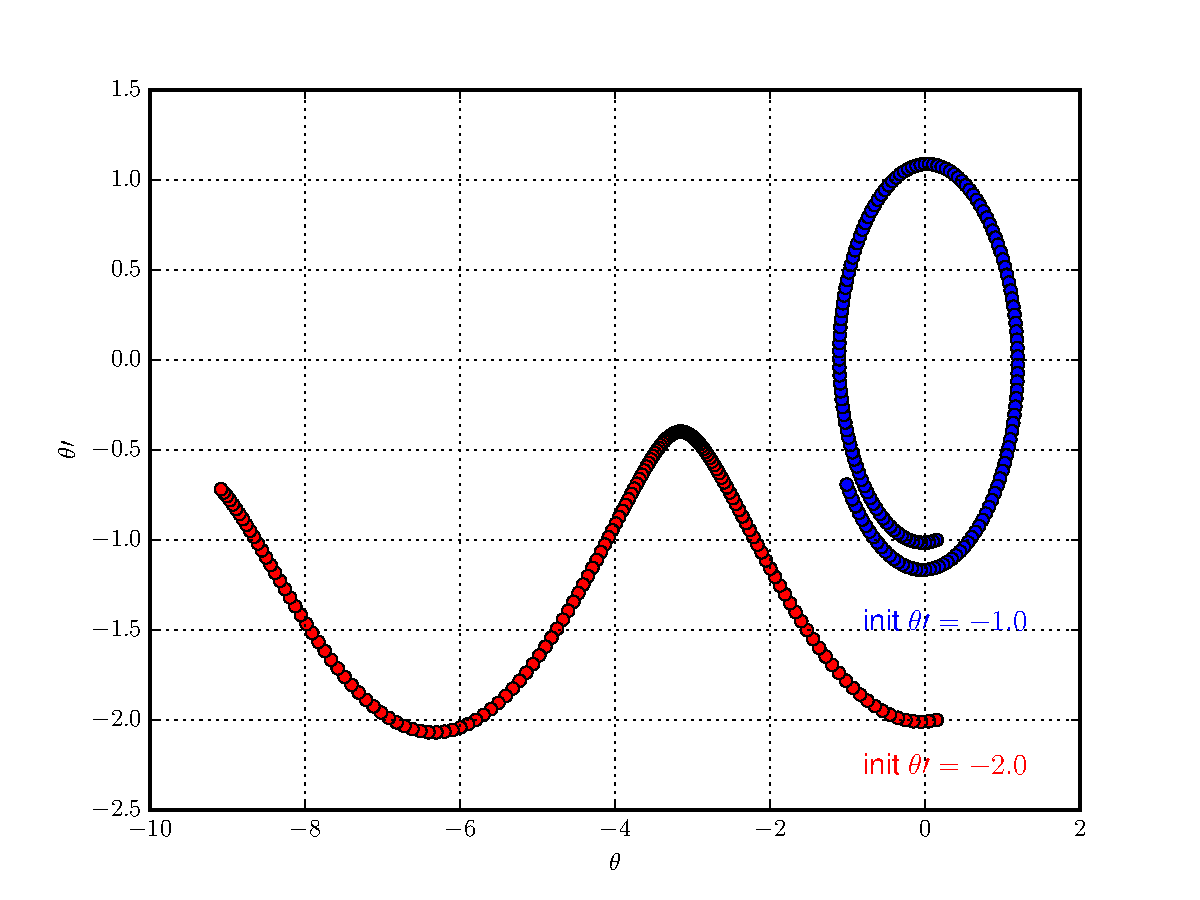
\includegraphics[width=7cm]{./resolnumeqdiff_1_fig.pdf}
\end{figure}
Ce genre de graphique s'appelle un portrait de phase.\newline
Quel est l'effet d'un changement d'unité ?
\end{frame}

\end{document}
